\documentclass{beamer}

\mode<presentation>
{
  \usetheme{default}      
  \usecolortheme{default}
  \usefonttheme{default}  
  \setbeamertemplate{navigation symbols}{}
  \setbeamertemplate{caption}[numbered]
} 

\usepackage[english]{babel}
\usepackage[utf8x]{inputenc}

\title[presentationTemplate]{An equilibrium theorem in non-linear population matrix models}
\author{Mark Alexander Burgess\\$ $\\Australian National University\\mark.burgess@anu.edu.au}
\date{\today}

\usepackage{amsthm, amssymb, amsfonts, amsmath}
\usepackage{graphicx}
\usepackage{tikz}
\usetikzlibrary{calc,shapes}
% \usepackage{enumitem}
\usepackage{mathtools}
\usepackage{mathrsfs}
\usepackage{tikz-cd}
\usepackage{MnSymbol,wasysym}
\usepackage{xcolor}
\usepackage{stackengine}


\newcommand\blfootnote[1]{%
  \begingroup
  \renewcommand\thefootnote{}\footnote{#1}%
  \addtocounter{footnote}{-1}%
  \endgroup
}

\newcommand{\C}{\mathbb{C}}
\newcommand{\R}{\mathbb{R}}
\newcommand{\Q}{\mathbb{Q}}
\newcommand{\Z}{\mathbb{Z}}
\newcommand{\N}{\mathbb{N}}
\newcommand{\p}{\mathbb{P}}
\newcommand{\E}{\mathbb{E}}

\begin{document}

\begin{frame}
  \titlepage
\end{frame}

\begin{frame}
\frametitle{Motivation}
To extend Evolutionary Game Theory, to model more things.
\end{frame}


\begin{frame}
\frametitle{Standard Evolutionary Game Theory}
\begin{itemize}
    \item fixed strategies
    \item stochastic pairing assumption
    \item fitness payoffs in a matrix
\end{itemize}
\-\\
eg. Hawk-Dove: Matrix and Replicator Equation
\begin{figure}
\centering
\begin{minipage}{5cm}
\begin{table}[]
\begin{tabular}{ccc}
                          & Hawk                         & Dove                     \\ \cline{2-3} 
\multicolumn{1}{c|}{Hawk} & \multicolumn{1}{c|}{V/2-C/2} & \multicolumn{1}{c|}{V}   \\ \cline{2-3} 
\multicolumn{1}{c|}{Dove} & \multicolumn{1}{c|}{0}       & \multicolumn{1}{c|}{V/2} \\ \cline{2-3} 
\end{tabular}
\end{table}
\end{minipage}
\begin{minipage}{5cm}
$ \dot{x}_i = x_i[f_i(x) - \phi(x)]$\\
$ \phi(x) = \sum_jx_jf_j(x)$
\end{minipage}
\end{figure}
Cost of Competition $C$, value of Resource $V$\\
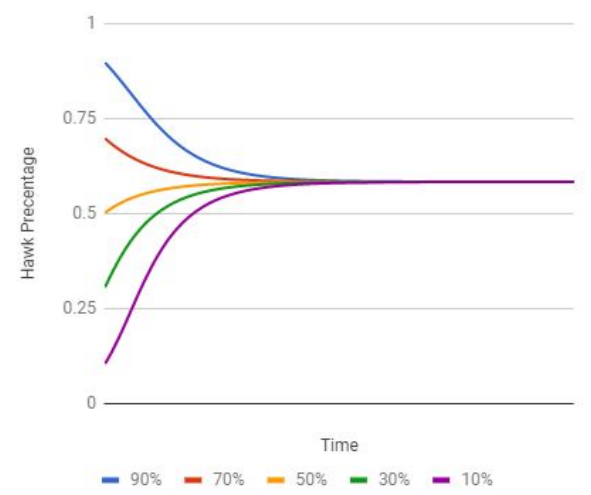
\includegraphics[width=60mm,height=40mm]{hawk_dove_graph.png}
\end{frame}




\begin{frame}
\frametitle{Motivation}
\begin{itemize}
\item Personal (Historic) Motivation: to evaluate evolutionary explanations about human psychology and behavior (Evolutionary Psychology).\\
%eg. Richard Dawkin's Optimal Coyness Game \cite{McNamara2009}  etc.
\end{itemize}
Criticism of evolutionary models:
\begin{itemize}
    \item Whatabout of factors. eg. environment, class, upbringing etc.
    \item The criticism of: unlikely evolutionary 'just-so' story.
\end{itemize}
Idea: lets model all the possible factors.
\end{frame}




\begin{frame}
\frametitle{Standard Evolutionary Game Theory?}
Problem:
\begin{table}[]
\begin{tabular}{lll}
                                & Psycho                   & non-Psycho               \\ \cline{2-3} 
\multicolumn{1}{l|}{Psycho}     & \multicolumn{1}{l|}{??}  & \multicolumn{1}{l|}{???} \\ \cline{2-3} 
\multicolumn{1}{l|}{non-Psycho} & \multicolumn{1}{l|}{1.2} & \multicolumn{1}{l|}{?}   \\ \cline{2-3} 
\end{tabular}
\end{table}
...What is the evolutionary fitness of Psychopathy?..
\-\\
\begin{figure}
\begin{minipage}{5cm}
--> it is: 1.08\\ \-\\
what are the units?
\end{minipage}
\begin{minipage}{5cm}
\begin{figure}
    \centering
    
\includegraphics{jason-voorhees.png}
\end{figure}
\end{minipage}
\end{figure}
\end{frame}






\begin{frame}
\frametitle{Standard Evolutionary Game Theory?}
Problem:
\begin{table}[]
\begin{tabular}{lll}
                                & Psycho                   & non-Psycho               \\ \cline{2-3} 
\multicolumn{1}{l|}{Psycho}     & \multicolumn{1}{l|}{??}  & \multicolumn{1}{l|}{???} \\ \cline{2-3} 
\multicolumn{1}{l|}{non-Psycho} & \multicolumn{1}{l|}{1.2} & \multicolumn{1}{l|}{?}   \\ \cline{2-3} 
\end{tabular}
\end{table}
What about:
\begin{itemize}
    \item Environment, Resource, Culture, Class, Randomness, Location, Mutation, Selection, Reciprocity
\end{itemize}
What is the evolutionary fitness of the peacock's tail?
how would we know? What would the number even mean?\-\\
Fitness values gloss over alot of possible factors.\\ \-\\
\blfootnote{https://plato.stanford.edu/entries/fitness/}
\end{frame}






\begin{frame}
%\frametitle{Standard Evolutionary Game Theory?}
{\huge ``Things are too simple....\\\-\hspace{1cm} Let us make them more complex"}\\\-\\\-\hspace{5cm}

\includegraphics[width=5cm,height=5cm]{thinking_emoji.png}
...yup...
\end{frame}





\begin{frame}
\frametitle{Artificial Life?}
Virtual Petri-dish; bots with code, replication and mutation:\\
Model as many factors as you like. But:\\
\begin{figure}
\begin{minipage}{5cm}
\begin{enumerate}
\item Results are stochastic
\item Difficult to generalize
\item hard to isolate cause and effect.
\item Interesting, but sometimes disappointing.
\end{enumerate}
\end{minipage}
\begin{minipage}{5cm}
\begin{figure}
    \centering
    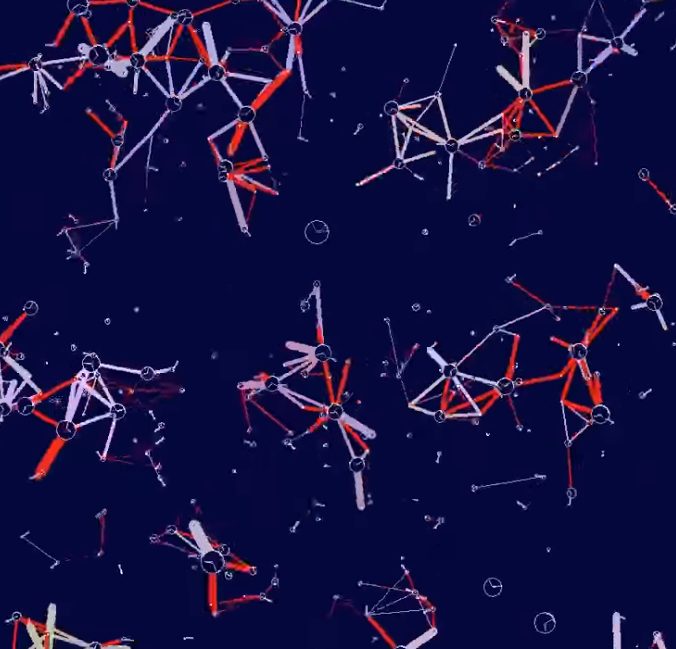
\includegraphics[width=5cm]{darwinbots_shot.png}
    \caption{Darwinbots\\http://wiki.darwinbots.com/}
\end{figure}
\end{minipage}
\end{figure}
\end{frame}




\begin{frame}
\frametitle{What did I do?}
\begin{enumerate}
\item I did research on Population Modelling and Game Theory
\item Investigated a Model for these questions, and made a general equilibrium theorem.
\item I moved on.
\end{enumerate}

\end{frame}




\begin{frame}
\frametitle{What have other people done?}
\begin{itemize}
\item Lots of work on Population Modelling.
\item Lots of work on Planning and Game-Theory (MDPs, and Stochastic-Games)
\item Lots of good work extending Game theory and evolutionary game theory to different environments, such as graphs and grids.
\item And lots of study about various evolutionary models.
\end{itemize}
\\\-\\
Specifically similar to: \\\-\\
Eitan Altman et.al \textit{Markov Decision Evolutionary Games}\\
Jim Michael (J. M.) Cushing \textit{Evolutionary Difference Equations}\\
Thomas L Vincent \textit{Evolutionary G-functions}\\
Hal Caswell\\
\end{frame}



\begin{frame}
\frametitle{Where do fitness values come from?}
Population Matrix models of \textit{vital rates} - eg. Leslie Matrix:
\begin{equation*}
\mathbf{M}=\begin{bmatrix}
    F_0 & F_1 & F_2 & \dots & F_{m-1} & F_m  \\
    P_0 &  0  &  0  & \dots &  0      &  0   \\
     0  & P_1 &  0  & \dots &  0      &  0   \\
     0  &  0  & P_2 & \dots &  0      &  0   \\
    \vdots & \vdots & \vdots & \ddots & \vdots & \vdots \\
     0  &  0  &  0  & \dots  & P_{m-1} &  0   \\
\end{bmatrix}
\end{equation*}
\begin{enumerate}
\item $P_i$ is probability of survival from the $i$th age bracket.\\
\item $F_i$ is number of offspring from the $i$th age bracket.\\
\end{enumerate}
For a population vector $\mathbf{n}(t)$ $$\mathbf{n}(t+1)=\mathbf{M}\mathbf{n}(t)$$
eventually a population profile $\mathbf{n}$ and a growth rate $\lambda$ as $\mathbf{M}\mathbf{n}=\lambda \mathbf{n}$.
\end{frame}





\begin{frame}
\begin{figure}[h]
        \centering
        \begin{tikzpicture}[scale=0.8, transform shape,->,>=stealth',shorten >=1pt,auto,node distance=1.7cm,thick,main node/.style={circle}]
            \path[use as bounding box] (-2.5cm, -2.8cm) rectangle (2.5cm, 2.5cm);
            \node[main node] (SB)  at (-2cm,  2cm) [align=center, text width=2.1cm] {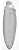
\includegraphics[width=.05\textwidth]{1.png}\\\small Seed};
            \node[main node] (SM)  at ( 2cm,  2cm) [align=center, text width=2.1cm] {
\includegraphics[width=.25\textwidth]{2.png}\\\small Small};
            \node[main node] (ME)  at ( 2cm, -2cm) [align=center, text width=2.1cm] {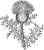
\includegraphics[width=.29\textwidth]{3.png}\\\small Medium};
            \node[main node] (LE)  at (-2cm, -2cm) [align=center, text width=2.1cm] {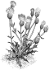
\includegraphics[width=.38\textwidth]{4.png}\\\small Large};

            \node[main node] (SBm) at (-2cm,  2cm) [align=center, text width=1.2cm] {};
            \node[main node] (SMm) at ( 2cm,  2cm) [align=center, text width=1.2cm] {};
            \node[main node] (MEm) at ( 2cm, -2cm) [align=center, text width=1.2cm] {};
            \node[main node] (LEm) at (-2cm, -2cm) [align=center, text width=1.2cm] {};

            \path[every node/.style={sloped,auto=false}]
            (SBm) edge [in=180-20,out=180+20,looseness=3,   line width=1pt,anchor=south] node  {\scriptsize 0.443} (SBm)
            (SBm) edge [bend left=15,                       line width=1pt,anchor=south] node  {\scriptsize 0.0039} (SMm)
            (SBm) edge [bend left=15,                       line width=1pt,anchor=south] node  {\scriptsize 0.0004} (MEm)
            (SBm) edge [bend left=15,                       line width=1pt,anchor=south] node  {\scriptsize 0.0005} (LEm)

            (SMm) edge [bend left=15,                       line width=1pt,anchor=south] node  {\scriptsize 0.1584} (SBm)
            (SMm) edge [in=20,out=-20,looseness=3,          line width=1pt,anchor=north] node  {\scriptsize 0.0078} (SMm)
            (SMm) edge [bend left=15,                       line width=1pt,anchor=south] node  {\scriptsize 0.0031} (MEm)
            (SMm) edge [bend left=15,                       line width=1pt,anchor=north] node  {\scriptsize 0.01} (LEm)

            (MEm) edge [bend left=15,                       line width=1pt,anchor=north] node  {\scriptsize 6.6105} (SBm)
            (MEm) edge [bend left=15,                       line width=1pt,anchor=south] node  {\scriptsize 0.2434} (SMm)
            (MEm) edge [in=-20,out=20,looseness=3,          line width=1pt,anchor=south] node  {\scriptsize 0.0314} (MEm)
            (MEm) edge [bend left=15,                       line width=1pt,anchor=south] node  {\scriptsize 0.0613} (LEm)

            (LEm) edge [bend left=15,                       line width=1pt,anchor=south] node  {\scriptsize 206.56} (SBm)
            (LEm) edge [bend left=15,                       line width=1pt,anchor=south] node  {\scriptsize 7.6091} (SMm)
            (LEm) edge [bend left=15,                       line width=1pt,anchor=south] node  {\scriptsize 0.793} (MEm)
            (LEm) edge [in=180+20,out=180-20,looseness=3,   line width=1pt,anchor=north] node  {\scriptsize 0.945} (LEm)
            ;
        \end{tikzpicture}
        $$ \begin{bmatrix}\text{Seed}_{t+1}\\\text{Small}_{t+1}\\\text{Medium}_{t+1}\\\text{Large}_{t+1}\end{bmatrix}= 
        \begin{bmatrix}
            0.443&0.1584&6.6105&206.56\\
            0.039&0.0078&0.2434&7.6091\\
            0.0004&0.0031&0.0314&0.793\\
            0.0005&0.01&0.0613&0.945
        \end{bmatrix}
        \begin{bmatrix}\text{Seed}_{t}\\\text{Small}_{t}\\\text{Medium}_{t}\\\text{Large}_{t}\end{bmatrix}$$
        \caption{
            4x4 matrix model of a Nodding Thistle (\textit{Carduus nutans}) population in Australia.
        }\label{fig:1b}
\end{figure}
\end{frame}







\begin{frame}
\frametitle{Where do fitness values come from?}
Population Matrix models of \textit{vital rates} - eg. Leslie Matrix:
\begin{equation*}
\mathbf{M}=\begin{bmatrix}
    F_0 & F_1 & F_2 & \dots & F_{m-1} & F_m  \\
    P_0 &  0  &  0  & \dots &  0      &  0   \\
     0  & P_1 &  0  & \dots &  0      &  0   \\
     0  &  0  & P_2 & \dots &  0      &  0   \\
    \vdots & \vdots & \vdots & \ddots & \vdots & \vdots \\
     0  &  0  &  0  & \dots  & P_{m-1} &  0   \\
\end{bmatrix}
\end{equation*}
$$\mathbf{n}(t+1)=\mathbf{M}\mathbf{n}(t)$$
\begin{figure}
%   \centering
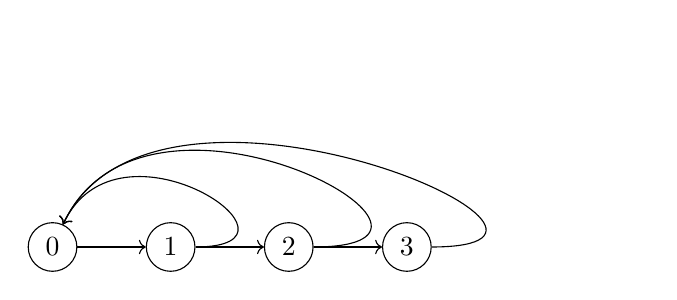
\begin{tikzpicture}
		\node [circle,draw] (1) at (0, 0) {0};
		\node [circle,draw] (2) at (1.5, 0) {1};
		\node [circle,draw] (3) at (3, 0) {2};
		\node [circle,draw] (4) at (4.5, 0) {3};
		%\node [circle,draw] (5) at (6, 0) {4};
		\draw [->] (1) to (2);
		\draw [->] (2) to (3);
		\draw [->] (3) to (4);
		%\draw [->] (4) to (5);
		
		\draw [->,out=0,in=65,looseness=2.5] (2) to (1);
		\draw [->,out=0,in=65,looseness=2.0] (3) to (1);
		\draw [->,out=0,in=65,looseness=1.5] (4) to (1);
		%\draw [->,out=0,in=65,looseness=1.3] (5) to (1);
\end{tikzpicture}
    \label{fig:my_label}
\end{figure}
\end{frame}















\begin{frame}
\frametitle{Introducing Strategies}
Alternative strategy has a different decision/action/policy giving different matrix column:
\begin{equation*}
\mathbf{M}=\begin{bmatrix}
    F_0 & F_1 & F_2 & F_3  \\
    P_0 &  0  &  0  &  0   \\
     0  & P_1 &  0  &  0   \\
     0  &  0  & P_2 &  0 
\end{bmatrix}
\qquad\qquad
\mathbf{M^*}=\begin{bmatrix}
    F_0 & \textcolor{red}{F^*_1} & F_2 & F_3  \\
    P_0 & \textcolor{red}{0}  &  0  &  0   \\
     0  & \textcolor{red}{P^*_1} &  0  &  0   \\
     0  & \textcolor{red}{0}  & P_2 &  0 
\end{bmatrix}
\end{equation*}
A mutation strategy will have growth-rates $\lambda$ and $\lambda^*$
\begin{figure}
    \centering
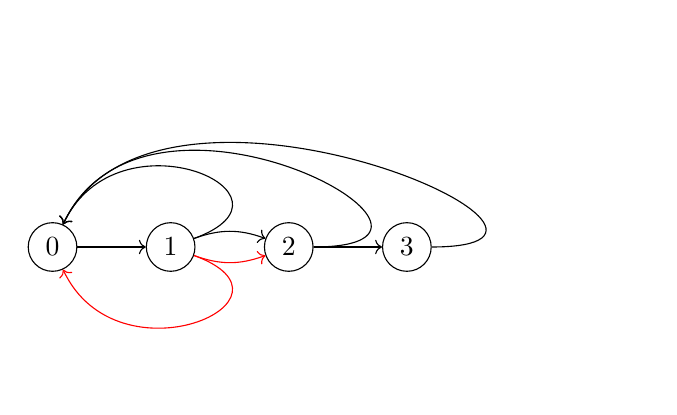
\begin{tikzpicture}
		\node [circle,draw] (1) at (0, 0) {0};
		\node [circle,draw] (2) at (1.5, 0) {1};
		\node [circle,draw] (3) at (3, 0) {2};
		\node [circle,draw] (4) at (4.5, 0) {3};
		%\node [circle,draw] (5) at (6, 0) {4};
		\draw [->] (1) to (2);
		\draw [->,out=20,in=160] (2) to (3);
		\draw [->,out=-20,in=-160,red] (2) to (3);
		\draw [->] (3) to (4);
		%\draw [->] (4) to (5);
		
		\draw [->,out=20,in=65,looseness=2.5] (2) to (1);
		\draw [->,red,out=-20,in=-65,looseness=2.5] (2) to (1);
		\draw [->,out=0,in=65,looseness=2.0] (3) to (1);
		\draw [->,out=0,in=65,looseness=1.5] (4) to (1);
		%\draw [->,out=0,in=65,looseness=1.3] (5) to (1);
\end{tikzpicture}
    \label{fig:my_label}
\end{figure}
\end{frame}



\begin{frame}
\frametitle{Introducing Strategies}
Mixed strategy has linear combination of matrix column:
\begin{equation*}
\mathbf{M}n=\begin{bmatrix}
    F_0 & F_1 & F_2 & F_3  \\
    P_0 &  0  &  0  &  0   \\
     0  & P_1 &  0  &  0   \\
     0  &  0  & P_2 &  0 
\end{bmatrix}n = \lambda n,
\quad
\mathbf{M^*}n^*=\begin{bmatrix}
    F_0 & \textcolor{red}{F^*_1} & F_2 & F_3  \\
    P_0 & \textcolor{red}{0}  &  0  &  0   \\
     0  & \textcolor{red}{P^*_1} &  0  &  0   \\
     0  & \textcolor{red}{0}  & P_2 &  0 
\end{bmatrix}n^*=\lambda^*n^*
\end{equation*}
mixing by $\textcolor{blue}{\alpha}$ gives a matrix
\begin{equation*}
\mathbf{M^\textcolor{blue}{\alpha}}n^{\textcolor{blue}{\alpha}}=\begin{bmatrix}
    F_0 & \textcolor{blue}{\alpha}F_1 + (1-\textcolor{blue}{\alpha})\textcolor{red}{F^*_1} & F_2 & F_3  \\
    P_0 & \textcolor{blue}{\alpha}0 + (1-\textcolor{blue}{\alpha})\textcolor{red}{0}  &  0  &  0   \\
     0  & \textcolor{blue}{\alpha}P_1 + (1-\textcolor{blue}{\alpha})\textcolor{red}{P^*_1} &  0  &  0   \\
     0  & \textcolor{blue}{\alpha}0 + (1-\textcolor{blue}{\alpha})\textcolor{red}{0}  & P_2 &  0 
\end{bmatrix}n^{\textcolor{blue}{\alpha}} = \lambda^{\textcolor{blue}{\alpha}}n^{\textcolor{blue}{\alpha}}
\end{equation*}
Each of these terms $P_0\dots P_n$ and $F_0\dots F_n$ are dependant on the population $n$.
Unstable if $\lambda^{\textcolor{blue}{\alpha}}>\lambda$ or $\frac{\partial \lambda^{\textcolor{blue}{\alpha}}}{\textcolor{blue}{\alpha}}\ne 0$ %\cite{Lebreton2000}
\end{frame}






\begin{frame}
\frametitle{Where do fitness values come from?}
For non-linear population models we make the Matrix a function of the population itself:
$$\mathbf{n}(t+1)=\mathbf{M}_{n(t)}\mathbf{n}(t)$$

\begin{itemize}
    \item Very general, can model a lot. (density dependant models, models of species, genetic combination, etc)
    \item even chaotic. (body of work on bifurcation)
\end{itemize}
We are interested in our equilibrium $\mathbf{M}_{n(t)}\mathbf{n}=\lambda \mathbf{n}$.

\begin{figure}
    \centering
    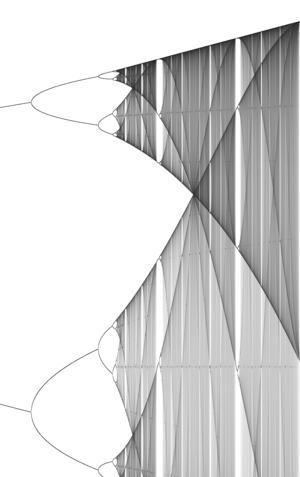
\includegraphics[width=7cm,height=10cm]{chaos.png}
    \caption{Caption}
    \label{fig:my_label}
\end{figure}
\end{frame}







\begin{frame}
\frametitle{Formalism}
\begin{itemize}
\item	$S$ be set of states
\item   $A_s$ be sets of actions at state $s\in S$
\item   $W$ be the set of strategies, $w_{a,s}$ denotes the probability of action $a$ in $s$.
\item	$P_{s,w}$ is the number of organisms in a state $s$ with strategy $w$;
\item   $P^*_{s,a} = \sum_{w\in W}P_{s,w}w_{a,s}$ is the number of organisms in a state $s$ which are going to take action $a$.
\item   $T_{s,a}(P^*)$ are vital rates depending, to state $s$ when execute an action $a$.
\end{itemize}

Thus every strategy $w$ has its own population matrix $\mathbf{M}_{P^*}^w$ with components $M^{w}_{i,j}$.%, and population vector $\mathbf{n}^w$.
\begin{equation}\label{eq:transmission_matrix}\mathbf{M}_{P^*}^w = M^{w}_{i,j} = \sum_{a\in A_i}T_{j,a}(P^*) w_{a,i}\end{equation}
\end{frame}





\begin{frame}
\frametitle{Equilibrium}
Equilibrium Definition:
\begin{itemize}
    \item For every strategy has a constant matrix $M^w_{P^*}$.
    \item Every strategy present ($P_{s,w}>0$) is growing/decaying at the same rate maximal $\lambda$.
\end{itemize}
Define an equilibrium point by $P^*$
\end{frame}


\begin{frame}
\frametitle{Central Theorem}
\fbox{%
\parbox{0.9\linewidth}{%
For every stable equilibrium point defined by $P^*$ established by mixed strategies, there is a set of pure strategies which give the same equilibrium point $P^*$.
}%
}\\\-\\\-\\
Ie. looking for equilibrium - you don't need to worry about mixed strategies.
\end{frame}



%\begin{frame}
%\frametitle{Proof part 1}
%
%\begin{equation*}
%\begin{bmatrix}
%    F_0 & F_1 & F_2 & F_3  \\
%    P_0 &  0  &  0  &  0   \\
%     0  & P_1 &  0  &  0   \\
%     0  &  0  & P_2 &  0 
%\end{bmatrix}
%\Rightarrow\quad \Rightarrow\quad\textcolor{blue}{\alpha}\quad \Rightarrow\quad \Rightarrow
%\begin{bmatrix}
%    F_0 & \textcolor{red}{F^*_1} & F_2 & F_3  \\
%    P_0 & \textcolor{red}{0}  &  0  &  0   \\
%     0  & \textcolor{red}{P^*_1} &  0  &  0   \\
%     0  & \textcolor{red}{0}  & P_2 &  0 
%\end{bmatrix}
%\end{equation*}
%If $\lambda_{\textcolor{blue}{\alpha}=0}=\lambda_{\textcolor{blue}{\alpha}=1}$ then %$\lambda_{\textcolor{blue}{\alpha}}=\lambda$ for all $\textcolor{blue}{\alpha}\in\mathbb{R}$.
%\begin{equation*}
%\begin{bmatrix}
%    F_0 & \textcolor{blue}{\alpha}F_1 + (1-\textcolor{blue}{\alpha})\textcolor{red}{F^*_1} & F_2 & F_3  \\
%    P_0 & \textcolor{blue}{\alpha}0 + (1-\textcolor{blue}{\alpha})\textcolor{red}{0}  &  0  &  0   \\
%     0  & \textcolor{blue}{\alpha}P_1 + (1-\textcolor{blue}{\alpha})\textcolor{red}{P^*_1} &  0  &  0   \\
%     0  & \textcolor{blue}{\alpha}0 + (1-\textcolor{blue}{\alpha})\textcolor{red}{0}  & P_2 &  0 
%\end{bmatrix}
%\end{equation*}
%\blfootnote{%oddblog.info/files/matrix\_equilibrium.pdf%\\
%preprints.org/manuscript/201703.0234
%}
%\end{frame}



%\begin{frame}
%\frametitle{Proof part 1}
%$$ \det(A-\lambda I)=\det(A^{b,k}-\lambda I)=0 \Rightarrow \det(\alpha A + (1-\alpha)A^{b,k}-\lambda %I)=0 $$
%
%determinant Cofactor expansion on the $k$th row:
%$$ 
%\stackinset{c}{}{c}{1.6\baselineskip}{\rule{4.4\baselineskip}{.4pt}}{%
%\stackinset{c}{.61\baselineskip}{c}{}{\rule{.4pt}{4.0\baselineskip}}{%
%\begin{pmatrix}
%        2 & 6 & 0 & 4\\
%        3 & 5 & 5 & 0\\
%        1 & 0 & 2 & 4\\
%        5 & 2 & 1 & 0\\
%\end{pmatrix}}}
%$$
%\blfootnote{https://www.preprints.org/manuscript/201703.0234}
%\end{frame}




\begin{frame}
\frametitle{Proof part 1\&2}
%For non-negative matrix $A$, and non-negative column vector $b$, with $A^{b,k}$ denoting the matrix with its $k$th column as $b$.
%For $B(\alpha) = \alpha A + (1-\alpha)A^{b,k}$ defined on a range $0\le\alpha\le1$.\\If $\rho(B(\alpha))$ is spectral radius.\\ Then $\rho(B(\alpha))$ is continuous, and either constant or strictly monotonic with $\alpha$.


\begin{equation*}
\begin{bmatrix}
    F_0 & F_1 & F_2 & F_3  \\
    P_0 &  0  &  0  &  0   \\
     0  & P_1 &  0  &  0   \\
     0  &  0  & P_2 &  0 
\end{bmatrix}
\Rightarrow\quad \Rightarrow\quad\textcolor{blue}{\alpha}\quad \Rightarrow\quad \Rightarrow
\begin{bmatrix}
    F_0 & \textcolor{red}{F^*_1} & F_2 & F_3  \\
    P_0 & \textcolor{red}{0}  &  0  &  0   \\
     0  & \textcolor{red}{P^*_1} &  0  &  0   \\
     0  & \textcolor{red}{0}  & P_2 &  0 
\end{bmatrix}
\end{equation*}

$\lambda_{\textcolor{blue}{\alpha}}$ is strictly monotonic or constant.\\\-\\
Either goes up \nearrow goes down \searrow stays constant \rightarrow\\
Does not go up and down \rightsquigarrow.\\\-\\

%continuous matrix = continuous eigenvalues, Perron-Frobenius theorem, intermediate value theorem.

\blfootnote{%oddblog.info/files/matrix\_equilibrium.pdf%\\
preprints.org/manuscript/201703.0234
}
\end{frame}




\begin{frame}
\frametitle{Proof part 3}

\begin{equation*}
\begin{bmatrix}
    F_0 & F_1 & F_2 & F_3  \\
    P_0 &  0  &  0  &  0   \\
     0  & P_1 &  0  &  0   \\
     0  &  0  & P_2 &  0 
\end{bmatrix}
\Rightarrow\quad \Rightarrow\quad\textcolor{blue}{\alpha}\quad \Rightarrow\quad \Rightarrow
\begin{bmatrix}
    F_0 & \textcolor{red}{F^*_1} & F_2 & F_3  \\
    P_0 & \textcolor{red}{0}  &  0  &  0   \\
     0  & \textcolor{red}{P^*_1} &  0  &  0   \\
     0  & \textcolor{red}{0}  & P_2 &  0 
\end{bmatrix}
\end{equation*}

If $\lambda_{\textcolor{blue}{\alpha}}$ is constant then there is a corresponding linearly changing eigenvector $n_{{\textcolor{blue}{\alpha}}} = {\textcolor{blue}{\alpha}}n_{{\textcolor{blue}{\alpha}}} + (1-{\textcolor{blue}{\alpha}}) n_{{\textcolor{blue}{\alpha}}}$; and the $\textcolor{red}{k}$th value is constant.\\\-\\

%Assumption of non-defective matrix.

\blfootnote{%oddblog.info/files/matrix\_equilibrium.pdf%\\
preprints.org/manuscript/201703.0234
}
\end{frame}





\begin{frame}
\frametitle{Proof part 4}
We can decompose mixed strategies into pure ones on the $\textcolor{red}{k}$th column.\\\-\\
\begin{figure}

\begin{minipage}{5cm}
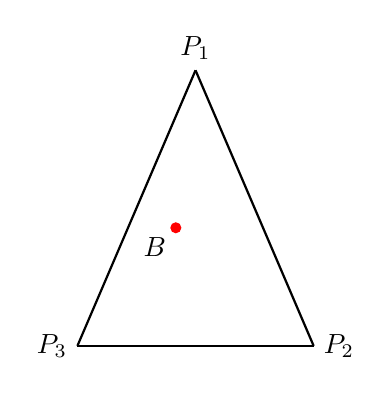
\begin{tikzpicture}[
    scale=5,
    important line/.style={thick},
    dashed line/.style={dashed, thin},
    pile/.style={thick, ->, >=stealth', shorten <=2pt, shorten
    >=2pt},
    every node/.style={color=black}
    ]
    % Lines
    \draw[important line] (.15+0.4,.15) coordinate (A) -- (.85,.85)
        coordinate (B) node[above] {$P_1$};
    \draw[important line] (0.85,.85) coordinate (C) -- (1.55-0.4,.15)
        coordinate (D) node[right] {$P_2$};
    \draw[important line] (1.55-0.4,.15) coordinate (G) -- (.15+0.4,.15)
        coordinate (H) node[left] {$P_3$};
    % The E point is placed more or less randomly
    \fill[red]  (A) +(+.25cm,+0.3cm) coordinate (out) circle (.4pt)
        node[below left] {$B$};
    % Line connecting out and ext balances
    %\draw [pile] (out) -- (intersection of A--B and out--[shift={(0:1pt)}]out) coordinate (extbal);
    %\fill[red] (extbal) circle (.4pt) node[above] {$C$};
    % line connecting  out and int balances
    %\draw [pile] (out) -- (intersection of C--D and out--[shift={(0:1pt)}]out) coordinate (intbal);
    %\fill[red] (intbal) circle (.4pt) node[above] {$D$};
    % line between out og all balanced out :)
    %\draw[pile] (out) -- (E);
\end{tikzpicture}
\end{minipage}
\begin{minipage}{5cm}
\begin{enumerate}
\item Mixed strategy internal to simplex.
%\item Difficult to generalize
%\item hard to isolate cause and effect.
%\item Interesting, but sometimes disappointing.
\end{enumerate}
\end{minipage}
\end{figure}
\blfootnote{%oddblog.info/files/matrix\_equilibrium.pdf%\\
preprints.org/manuscript/201703.0234
}
\end{frame}





\begin{frame}
\frametitle{Proof part 4}
We can decompose mixed strategies into pure ones on the $\textcolor{red}{k}$th column.\\\-\\
\begin{figure}

\begin{minipage}{5cm}
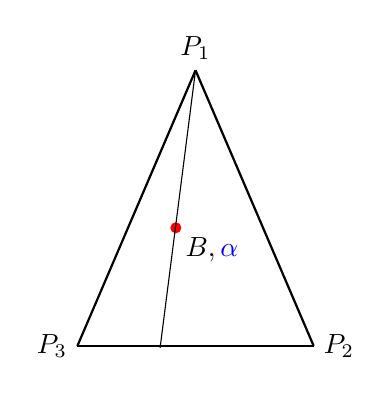
\begin{tikzpicture}[
    scale=5,
    important line/.style={thick},
    dashed line/.style={dashed, thin},
    pile/.style={thick, ->, >=stealth', shorten <=2pt, shorten
    >=2pt},
    every node/.style={color=black}
    ]
    % Lines
    \draw[important line] (.15+0.4,.15) coordinate (A) -- (.85,.85)
        coordinate (B) node[above] {$P_1$};
    \draw[important line] (0.85,.85) coordinate (C) -- (1.55-0.4,.15)
        coordinate (D) node[right] {$P_2$};
    \draw[important line] (1.55-0.4,.15) coordinate (G) -- (.15+0.4,.15)
        coordinate (H) node[left] {$P_3$};
    % The E point is placed more or less randomly
    \fill[red]  (A) +(+.25cm,+0.3cm) coordinate (out) circle (.4pt)
        node[below right] {$B,{\textcolor{blue}{\alpha}}$};
    \draw (B)--(0.76,0.145);
    % Line connecting out and ext balances
    %\draw [pile] (out) -- (intersection of A--B and out--[shift={(0:1pt)}]out) coordinate (extbal);
    %\fill[red] (extbal) circle (.4pt) node[above] {$C$};
    % line connecting  out and int balances
    %\draw [pile] (out) -- (intersection of C--D and out--[shift={(0:1pt)}]out) coordinate (intbal);
    %\fill[red] (intbal) circle (.4pt) node[above] {$D$};
    % line between out og all balanced out :)
    %\draw[pile] (out) -- (E);
\end{tikzpicture}
\end{minipage}
\begin{minipage}{5cm}
\begin{enumerate}
\item Mixed strategy internal to simplex.
\item consider linear relation between $B$ and $P_1$
%\item hard to isolate cause and effect.
%\item Interesting, but sometimes disappointing.
\end{enumerate}
\end{minipage}
\end{figure}
\blfootnote{%oddblog.info/files/matrix\_equilibrium.pdf%\\
preprints.org/manuscript/201703.0234
}
\end{frame}





\begin{frame}
\frametitle{Proof part 4}
We can decompose mixed strategies into pure ones on the $\textcolor{red}{k}$th column.\\\-\\
\begin{figure}

\begin{minipage}{5cm}
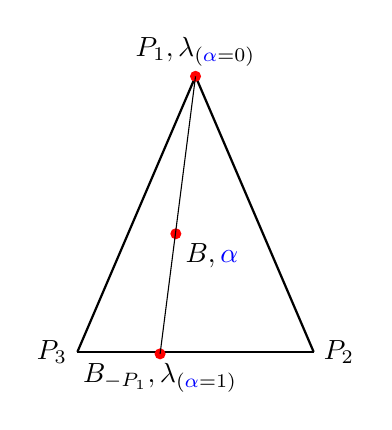
\begin{tikzpicture}[
    scale=5,
    important line/.style={thick},
    dashed line/.style={dashed, thin},
    pile/.style={thick, ->, >=stealth', shorten <=2pt, shorten
    >=2pt},
    every node/.style={color=black}
    ]
    % Lines
    \draw[important line] (.15+0.4,.15) coordinate (A) -- (.85,.85)
        coordinate (B) node[above] {$P_1,\lambda_{({\textcolor{blue}{\alpha}}=0)}$};
    \draw[important line] (0.85,.85) coordinate (C) -- (1.55-0.4,.15)
        coordinate (D) node[right] {$P_2$};
    \draw[important line] (1.55-0.4,.15) coordinate (G) -- (.15+0.4,.15)
        coordinate (H) node[left] {$P_3$};
    % The E point is placed more or less randomly
    \fill[red]  (B) coordinate (out) circle (.4pt)
        node[below left] {};
    \fill[red]  (0.76,0.145) coordinate (out) circle (.4pt)
        node[below] {$B_{-P_1},\lambda_{({\textcolor{blue}{\alpha}}=1)}$};
    \fill[red]  (A) +(+.25cm,+0.3cm) coordinate (out) circle (.4pt)
        node[below right] {$B,{\textcolor{blue}{\alpha}}$};
    \draw (B)--(0.76,0.145);
    % Line connecting out and ext balances
    %\draw [pile] (out) -- (intersection of A--B and out--[shift={(0:1pt)}]out) coordinate (extbal);
    %\fill[red] (extbal) circle (.4pt) node[above] {$C$};
    % line connecting  out and int balances
    %\draw [pile] (out) -- (intersection of C--D and out--[shift={(0:1pt)}]out) coordinate (intbal);
    %\fill[red] (intbal) circle (.4pt) node[above] {$D$};
    % line between out og all balanced out :)
    %\draw[pile] (out) -- (E);
\end{tikzpicture}
\end{minipage}
\begin{minipage}{5cm}
\begin{enumerate}
\item Mixed strategy internal to simplex.
\item consider linear relation between $B$ and $P_1$
\item if $\lambda$ is increasing or decreasing along the line then not equilibrium
\item otherwise $\lambda$ constant, and decompose population eigenvectors into pure strategies at $P_1$ and $B_{-P_1}$.
\end{enumerate}
\end{minipage}
\end{figure}
\blfootnote{%oddblog.info/files/matrix\_equilibrium.pdf%\\
preprints.org/manuscript/201703.0234
}
\end{frame}





\begin{frame}
\frametitle{Proof part 5}
Decompose mixed strategies into pure ones on the $\textcolor{red}{k}$th column.\\\-\\
And decompose each of them into pure ones on the $\textcolor{red}{k+1}$th column.\\\-\\
And decompose each of them into pure ones on the $\textcolor{red}{k+2}$th column.\\\-\\
.........

\blfootnote{%oddblog.info/files/matrix\_equilibrium.pdf%\\
preprints.org/manuscript/201703.0234
}
\end{frame}




\begin{frame}
\frametitle{Central Theorem}
\fbox{%
\parbox{0.9\linewidth}{%
For every stable equilibrium point defined by $P^*$ established by mixed strategies, there is a set of pure strategies which give the same equilibrium point $P^*$.
}%
}\\\-\\\-\\
Ie. looking for equilibrium - you don't need to worry about mixed strategies (eliminates a lot of strategies).\\\-\\
Redundancy of mixed strategies is not true for disequilibrium.\\\-\\
basic statement for such a general system. wont help you find equilibrium though.\\
\end{frame}







\begin{frame}
\frametitle{illustration}
\begin{figure}
    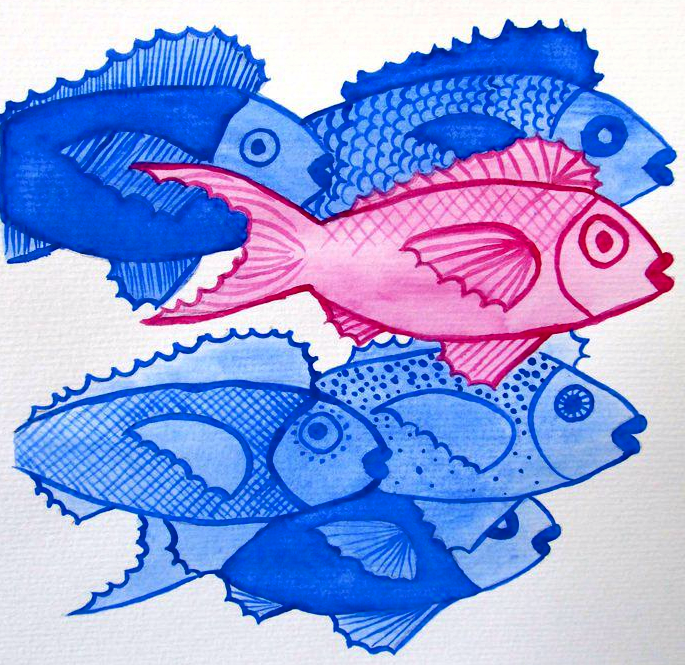
\includegraphics[width=5cm,height=5cm]{school1.png}
    \label{fig:my_label}
\end{figure}
School of indistinguishable fish, half gradually turn red at adolescence.\\
A case with 100\% of the population having a gene with 50\% chance turning red. Is indistinguishable from 50\% of the population population having a gene of 100\% chance turning red. No matter what.
\end{frame}





\begin{frame}
Any Questions?

\blfootnote{
preprints.org/manuscript/201703.0234\\mark.burgess@anu.edu.au
}

\end{frame}





\begin{frame}
\frametitle{Limitations}
\begin{itemize}
    \item Assume all relevant mutations already exist (no direct modeling of mutation)
    \item No direct modeling of environment (though easily remedied) $$T_{s,a}(P^*,\textcolor{blue}{E}),\qquad\mathbf{n}(t+1)=\mathbf{M}_{n(t),\textcolor{blue}{E}}\mathbf{n}(t)$$
    \item continuous populations, nothing stochastic.
    \item Proofs assume exponential growth rates: $\mathbf{M}_{n(t)}\mathbf{n}=\lambda \mathbf{n}$, but some matrices are defective.
\begin{equation}
\begin{bmatrix}
1&1\\
0&1
\end{bmatrix}
,\qquad 
\begin{bmatrix}
1\\
1
\end{bmatrix},
\begin{bmatrix}
2\\
1
\end{bmatrix},
\begin{bmatrix}
3\\
1
\end{bmatrix},
\begin{bmatrix}
4\\
1
\end{bmatrix},\dots
\end{equation}
Suspicion still holds, but potentially unphysical.
\end{itemize}
\end{frame}




\begin{frame}
\frametitle{Relation to Other Approaches}
Other approaches are so close!!!
\begin{enumerate}
    \item Some (eg. MDEG) model an 'inner' and 'outer' evolutionary game. can be approximated by $$ \mathbf{M}_{n(t)} = \mathbf{T}_{n(t)}+\textcolor{blue}{\epsilon}\mathbf{R}_{n(t)}$$
    \item Other's analyse Evolutionary change by hill-climbing on adaptive landscape, G-matricies and Lande's equations, some game-theory, but not necessarily state-based.
    \item Other approaches emphasize stability of matricies $\partial \lambda=0$ including perturbation analysis, Takada-Nakajima equation, but don't quite go full game theory %\cite{Takada1992,Takada1998}
\end{enumerate}
\end{frame}





% \begin{frame}
% % \frametitle{d}
%    \onslide<1->{
%    } % onslide 2
%    \onslide<1->{
%    } % onslide 3
%    \onslide<1->{
%    } % onslide 4
%    \onslide<1->{
%    } % onslide 5
%    \onslide<1->{
%    } % onslide 6
%    \onslide<1->{
%    } % onslide 7
%    \onslide<1->{
%    } % onslide 8
%    \onslide<1->{
%    } % onslide 9
%    \onslide<1->{
%    } % onslide 10
% \end{frame}


% \begin{frame}
% % \frametitle{d}
%    \onslide<1->{
%    } % onslide 2
%    \onslide<1->{
%    } % onslide 3
%    \onslide<1->{
%    } % onslide 4
%    \onslide<1->{
%    } % onslide 5
%    \onslide<1->{
%    } % onslide 6
%    \onslide<1->{
%    } % onslide 7
%    \onslide<1->{
%    } % onslide 8
%    \onslide<1->{
%    } % onslide 9
%    \onslide<1->{
%    } % onslide 10
% \end{frame}



% \begin{frame}
% % \frametitle{d}
%    \onslide<1->{
%    } % onslide 2
%    \onslide<1->{
%    } % onslide 3
%    \onslide<1->{
%    } % onslide 4
%    \onslide<1->{
%    } % onslide 5
%    \onslide<1->{
%    } % onslide 6
%    \onslide<1->{
%    } % onslide 7
%    \onslide<1->{
%    } % onslide 8
%    \onslide<1->{
%    } % onslide 9
%    \onslide<1->{
%    } % onslide 10
% \end{frame}



% \begin{frame}
% % \frametitle{d}
%    \onslide<1->{
%    } % onslide 2
%    \onslide<1->{
%    } % onslide 3
%    \onslide<1->{
%    } % onslide 4
%    \onslide<1->{
%    } % onslide 5
%    \onslide<1->{
%    } % onslide 6
%    \onslide<1->{
%    } % onslide 7
%    \onslide<1->{
%    } % onslide 8
%    \onslide<1->{
%    } % onslide 9
%    \onslide<1->{
%    } % onslide 10
% \end{frame}



% \begin{frame}
% % \frametitle{d}
%    \onslide<1->{
%    } % onslide 2
%    \onslide<1->{
%    } % onslide 3
%    \onslide<1->{
%    } % onslide 4
%    \onslide<1->{
%    } % onslide 5
%    \onslide<1->{
%    } % onslide 6
%    \onslide<1->{
%    } % onslide 7
%    \onslide<1->{
%    } % onslide 8
%    \onslide<1->{
%    } % onslide 9
%    \onslide<1->{
%    } % onslide 10
% \end{frame}



\end{document}
